\documentclass[11pt,a4paper]{article}

\usepackage{fontspec}
\usepackage{polyglossia}
\setdefaultlanguage{french}

\usepackage{graphicx}
\usepackage{amsmath, amssymb}
\usepackage{geometry}
\usepackage{hyperref}
\usepackage{enumitem}
\usepackage{booktabs}
\usepackage{array}
\usepackage{xcolor}
\usepackage{float}
\usepackage{listings}

\geometry{margin=2.5cm}
\setlength{\parindent}{0pt}
\setlength{\parskip}{6pt}
\setlist[itemize]{leftmargin=1.2cm, itemsep=2pt, topsep=4pt}

\hypersetup{colorlinks=true, linkcolor=black, urlcolor=blue}

\definecolor{codegray}{gray}{0.95}
\definecolor{codekw}{rgb}{0.13,0.29,0.53}
\definecolor{codestr}{rgb}{0.58,0.00,0.00}
\definecolor{codecom}{rgb}{0.25,0.50,0.25}

\lstset{
    basicstyle=\ttfamily\footnotesize,
    backgroundcolor=\color{codegray},
    keywordstyle=\color{codekw}\bfseries,
    stringstyle=\color{codestr},
    commentstyle=\color{codecom}\itshape,
    breaklines=true,
    columns=fullflexible,
    frame=single,
    framesep=3pt,
    xleftmargin=5pt,
    showstringspaces=false,
    captionpos=b
}

\newcommand{\code}[1]{\texttt{#1}}
\newcommand{\todo}[1]{\textcolor{red}{\textbf{[TODO : #1]}}}

\begin{document}

\begin{titlepage}
    \begin{flushright}
        
\includegraphics[width=0.5\textwidth]{assets/UPC_Logo.png}
    \end{flushright}

    \vspace{2cm}
    \centering

    {\Huge\bfseries Rapport de projet\\[0.4cm]}
    {\LARGE Programmation distribuée\\[0.3cm]}
    {\Large EventHub -- Plateforme de gestion d'évènements\\ en architecture microservices\\[0.8cm]}

    {\large Mehdi AGHAEI\\[0.2cm]}
    {\large Maksym DOLHOV\\[0.2cm]}
    {\large Fallou DIOUF\\[0.6cm]}

    {\large M1 VMI\\[2.2cm]}
    {\large \today}
\end{titlepage}

\tableofcontents
\newpage

% ====================================================
\section{Introduction}

Le projet \textbf{EventHub} est une application web distribuée de gestion d'évènements mise en œuvre selon les contraintes technologiques imposées par le sujet de Programmation distribuée : architecture en microservices, conteneurisation avec Docker, orchestration avec Kubernetes, et passerelle d'entrée unique (gateway / ingress). Le choix d'un cas d'usage \emph{sujet libre} nous a orientés vers une plateforme simple mais fonctionnellement complète, proche d'un produit de type Meetup ou Eventbrite en version minimale, afin de rendre la séparation en microservices à la fois naturelle et pédagogiquement lisible.

Le travail a été mené en trinôme : \textbf{Mehdi AGHAEI}, \textbf{Maksym DOLHOV} et \textbf{Fallou DIOUF}. Les contributions ont été réparties autour de trois axes -- backend (services Django), frontend (React) et infrastructure (Docker, Kubernetes, sécurité) -- avec des revues croisées pour garantir la cohérence de l'ensemble.

Ce rapport est organisé selon la grille d'évaluation fournie dans le sujet, chaque section correspondant à un niveau de la montée en note (10/20, 12/20, 14/20, 16/20, 18/20, 20/20) et décrivant précisément ce qui a été livré à ce palier. Un chapitre final revient sur les critères d'évaluation (intégration technologique, codage, fonctionnalités, présentation).

\section{Contexte fonctionnel}

EventHub permet à des utilisateurs de s'inscrire, de se connecter, de parcourir une liste d'évènements classés par catégories, et de créer de nouveaux évènements. Les fonctionnalités principales sont volontairement limitées : l'objectif n'est pas de couvrir l'intégralité d'une plateforme commerciale, mais de disposer d'un domaine métier suffisamment riche pour justifier \emph{deux} microservices métier distincts avec des responsabilités claires et une base de données.

Périmètre fonctionnel livré :
\begin{itemize}
    \item inscription d'un utilisateur et connexion par JWT (access + refresh)
    \item consultation du profil authentifié
    \item création, listing, modification et suppression d'évènements
    \item gestion des catégories d'évènements
    \item interface web React consommant les deux APIs à travers la passerelle
\end{itemize}

% ====================================================
\section{Architecture et choix technologiques}

\subsection{Vue d'ensemble}

L'architecture est structurée autour de trois services applicatifs, une base de données partagée avec cloisonnement logique, et une passerelle en entrée :

\begin{verbatim}
                        Navigateur
                            |
                            v
                 +----------------------+
                 |  Gateway / Ingress   |   (Nginx local / Nginx Ingress K8s)
                 +----------------------+
                   /        |         \
                  /         |          \
         /events          /users          /
            |               |             |
            v               v             v
   +----------------+  +--------------+  +----------------+
   | event-service  |  | user-service |  | frontend (React)|
   |  Django REST   |  | Django REST  |  |   Vite + Nginx  |
   +----------------+  +--------------+  +----------------+
            \               /
             \             /
              v           v
           +--------------------+
           |   PostgreSQL 16    |
           |  (StatefulSet K8s) |
           +--------------------+
             bases : eventhub_events / eventhub_users
\end{verbatim}

Chaque microservice est indépendant en terme de code, de build et de cycle de vie. Ils ne se parlent pas directement entre eux : la cohésion se fait côté client (le frontend appelle les deux APIs via la gateway) et la séparation des responsabilités est renforcée par le fait que chaque backend ne voit \emph{que sa propre base logique} dans PostgreSQL.

\subsection{Choix des technologies}

\begin{table}[H]
\centering
\begin{tabular}{ll}
\toprule
Couche & Technologie retenue \\
\midrule
Microservices backend   & Python 3.12 + Django 5 + Django REST Framework \\
Authentification        & djangorestframework-simplejwt (JWT) \\
Frontend                & React 18 + Vite, servi par Nginx en production \\
Base de données         & PostgreSQL 16 (Alpine) \\
Conteneurisation        & Docker + Docker Compose (orchestration locale) \\
Orchestration cloud     & Kubernetes (cible Minikube + GKE compatible) \\
Gateway local           & Nginx 1.27 en reverse proxy \\
Gateway K8s             & Ingress NGINX Controller \\
Secrets / configuration & \code{Secret} + \code{ConfigMap} Kubernetes \\
Persistance             & \code{StatefulSet} PostgreSQL + PV/PVC \\
Sécurité cluster        & RBAC (\code{Role} + \code{RoleBinding}) \\
\bottomrule
\end{tabular}
\caption{Stack technique du projet EventHub.}
\end{table}

Le choix de Django pour les deux backends -- plutôt que de varier volontairement les langages -- est motivé par l'objectif pédagogique : dans un rendu de quelques semaines, multiplier les écosystèmes aurait dilué l'effort sur l'infrastructure alors que l'évaluation valorise l'\emph{intégration} des technologies imposées (Web Services, Docker, Kubernetes). Les deux services restent néanmoins indépendants, avec leurs propres \code{Dockerfile}, \code{requirements.txt} et base logique.

% ====================================================
\section{Palier 10/20 : un microservice, Docker, Kubernetes}

Le premier jalon du sujet consiste à livrer un service fonctionnel, conteneurisé, puis déployé sous Kubernetes. Nous avons commencé par le \code{event-service}.

\subsection{Le service \code{event-service}}

Le service expose une API REST pour la gestion des évènements et des catégories, avec les modèles \code{Event} et \code{Category} (clé étrangère nullable). Il utilise Django REST Framework et ses vues génériques pour les opérations CRUD.

Routes principales :
\begin{itemize}
    \item \code{GET / POST /events/}
    \item \code{GET / PUT / PATCH / DELETE /events/<id>/}
    \item \code{GET / POST /events/categories/}
    \item \code{GET /health/} -- endpoint de santé pour les probes
\end{itemize}

\subsection{Dockerfile et image}

L'image est construite à partir de \code{python:3.12-slim}, avec une étape d'installation des dépendances système (\code{gcc}, \code{libpq-dev}) nécessaires au pilote PostgreSQL, puis \code{pip install} des dépendances Python. Un script \code{entrypoint.sh} applique les migrations Django au démarrage avant de lancer Gunicorn.

\begin{lstlisting}[language=bash, caption={Construction et publication de l'image}]
docker build -t eventhub-event-service:latest ./services/event-service
docker tag  eventhub-event-service:latest 3v3r51nc3/eventhub-event-service:latest
docker push 3v3r51nc3/eventhub-event-service:latest
\end{lstlisting}

\subsection{Déploiement Kubernetes}

Le service est déployé via un \code{Deployment} mono-réplica et exposé en \code{ClusterIP}. La configuration est injectée via un \code{ConfigMap} (paramètres applicatifs) et un \code{Secret} (mot de passe base de données), ce qui évite toute fuite de secret dans les manifestes YAML.

\begin{lstlisting}[caption={Extrait de \code{k8s/event-deployment.yaml}}]
spec:
  containers:
    - name: event-service
      image: eventhub-event-service:latest
      imagePullPolicy: IfNotPresent
      envFrom:
        - configMapRef:
            name: event-config
      env:
        - name: DB_PASSWORD
          valueFrom:
            secretKeyRef:
              name: postgres-secret
              key: EVENT_DB_PASSWORD
\end{lstlisting}

\begin{figure}[H]
  \centering
  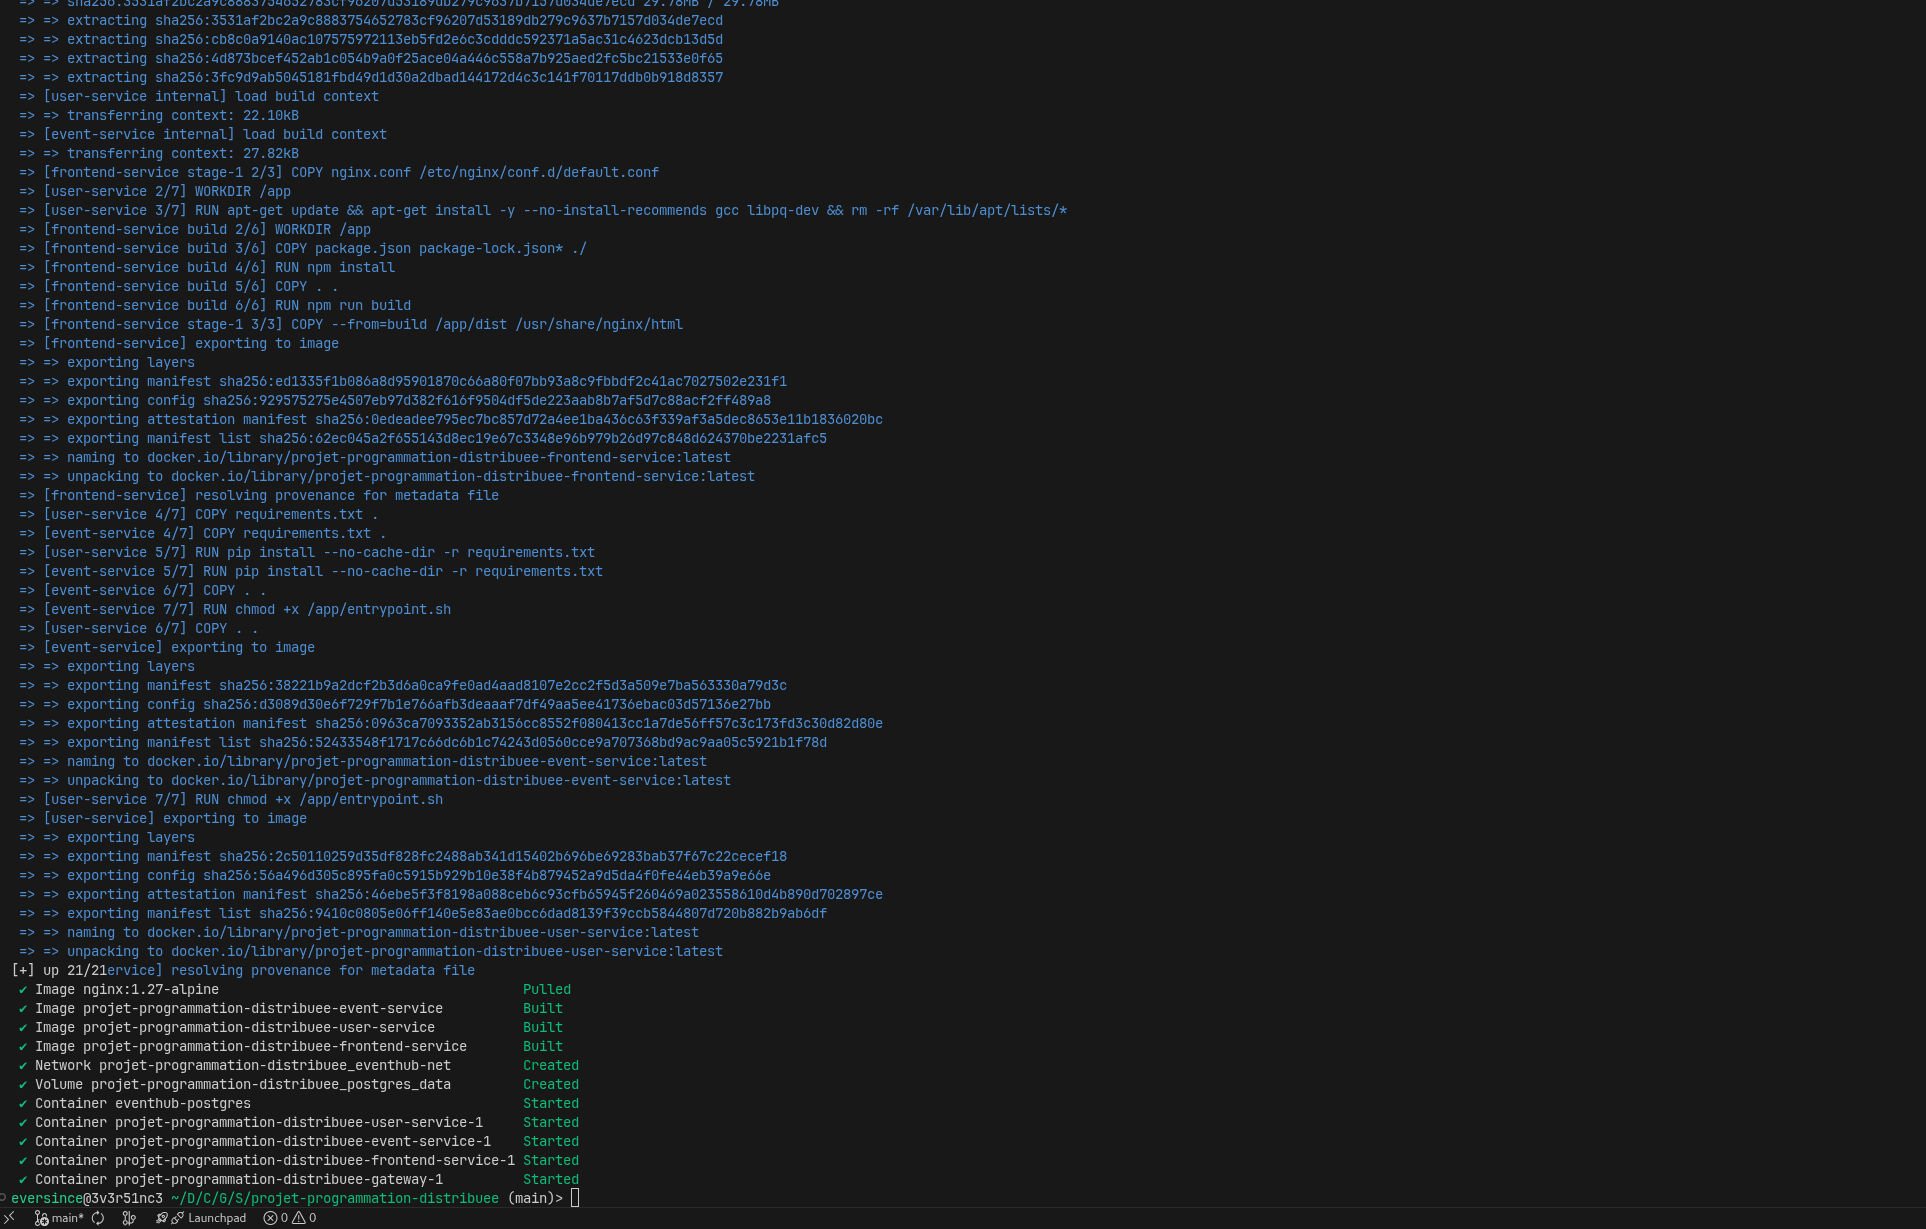
\includegraphics[width=\linewidth]{assets/screen-01-docker-compose.png}
  \caption{Les cinq conteneurs du projet en exécution via \code{docker compose up}.}
\end{figure}

\begin{figure}[H]
  \centering
  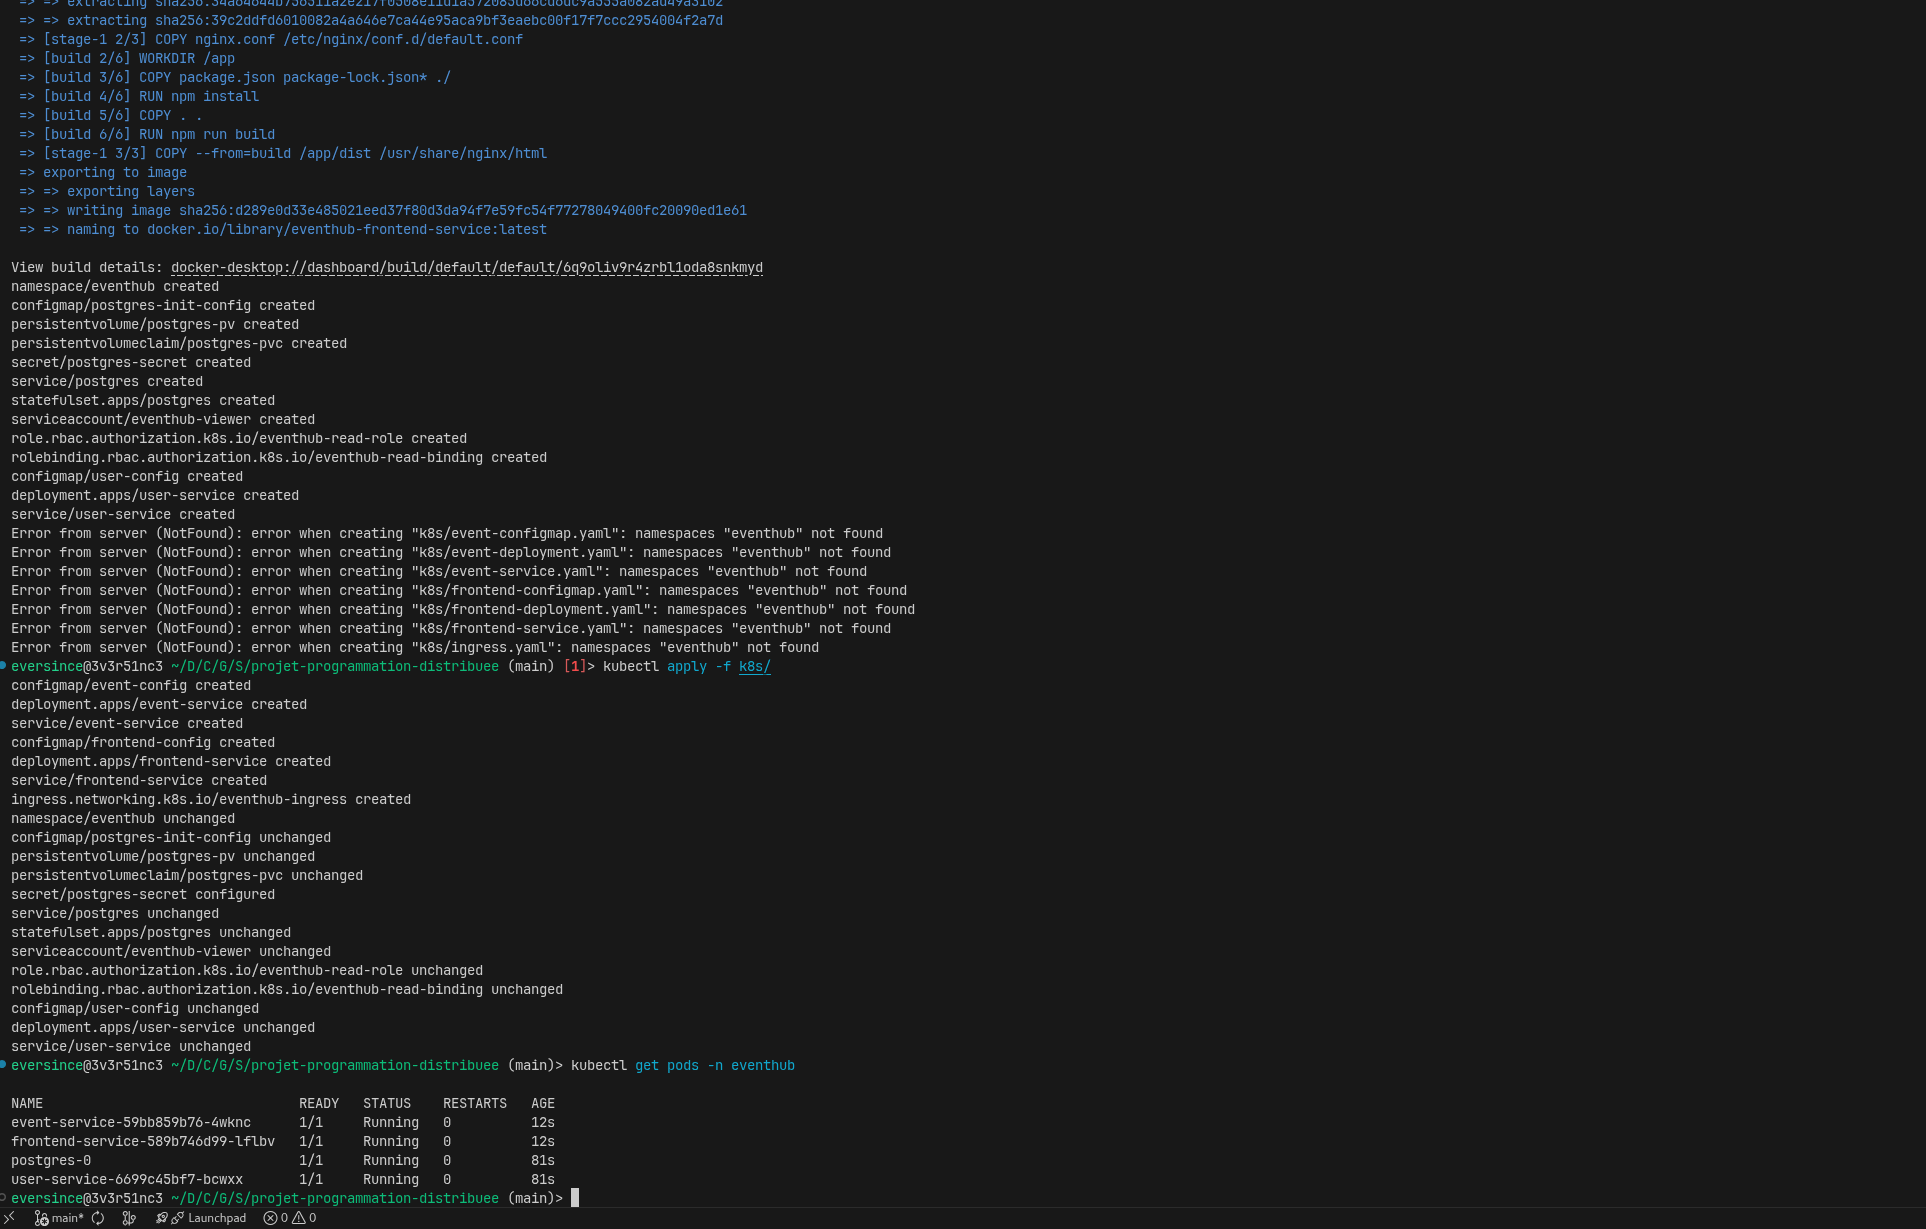
\includegraphics[width=\linewidth]{assets/screen-02-kubectl-pods-svc.png}
  \caption{\code{kubectl get pods,svc -n eventhub} -- \code{event-service} en état \code{Running}.}
\end{figure}

% ====================================================
\section{Palier 12/20 : une passerelle locale}

Le deuxième palier demande l'ajout d'une passerelle unique pour masquer la topologie interne des services. Nous avons adopté deux passerelles cohérentes :

\begin{itemize}
    \item \textbf{En local} : un service Nginx lancé par Docker Compose qui fait du reverse proxy sur les trois services (\code{/events}, \code{/users}, \code{/}).
    \item \textbf{En Kubernetes} : un objet \code{Ingress} basé sur le contrôleur NGINX (addon Minikube) qui réplique exactement la même logique de routage.
\end{itemize}

Cette symétrie est un choix assumé : un développeur peut tester localement via \code{docker compose up} exactement le même graphe d'URL que celui déployé en cluster, sans modifier la configuration frontend.

\begin{lstlisting}[caption={Extrait de \code{gateway/nginx.conf}}]
location /events/ {
    proxy_pass http://event-service:8000;
    proxy_set_header Host $host;
    proxy_set_header X-Forwarded-For $proxy_add_x_forwarded_for;
}
location /users/ {
    proxy_pass http://user-service:8000;
    ...
}
location / {
    proxy_pass http://frontend-service:80;
    ...
}
\end{lstlisting}

Côté Kubernetes, l'\code{Ingress} définit les mêmes trois règles sur l'hôte virtuel \code{eventhub.local}. Les services backend restent en \code{ClusterIP} : l'Ingress est \emph{le seul} point d'entrée public du cluster, ce qui est également un élément qui compte dans les paliers de sécurité (18/20).

\begin{figure}[H]
  \centering
  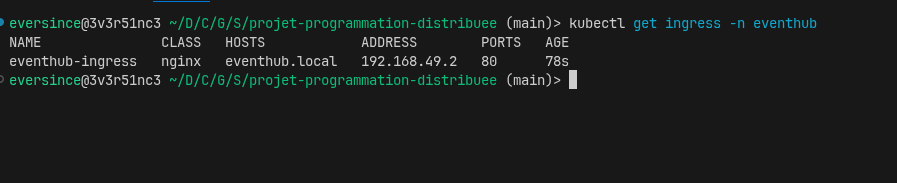
\includegraphics[width=\linewidth]{assets/screen-03-kubectl-ingress.png}
  \caption{\code{kubectl get ingress -n eventhub} -- l'Ingress NGINX avec son adresse.}
\end{figure}

\begin{figure}[H]
  \centering
  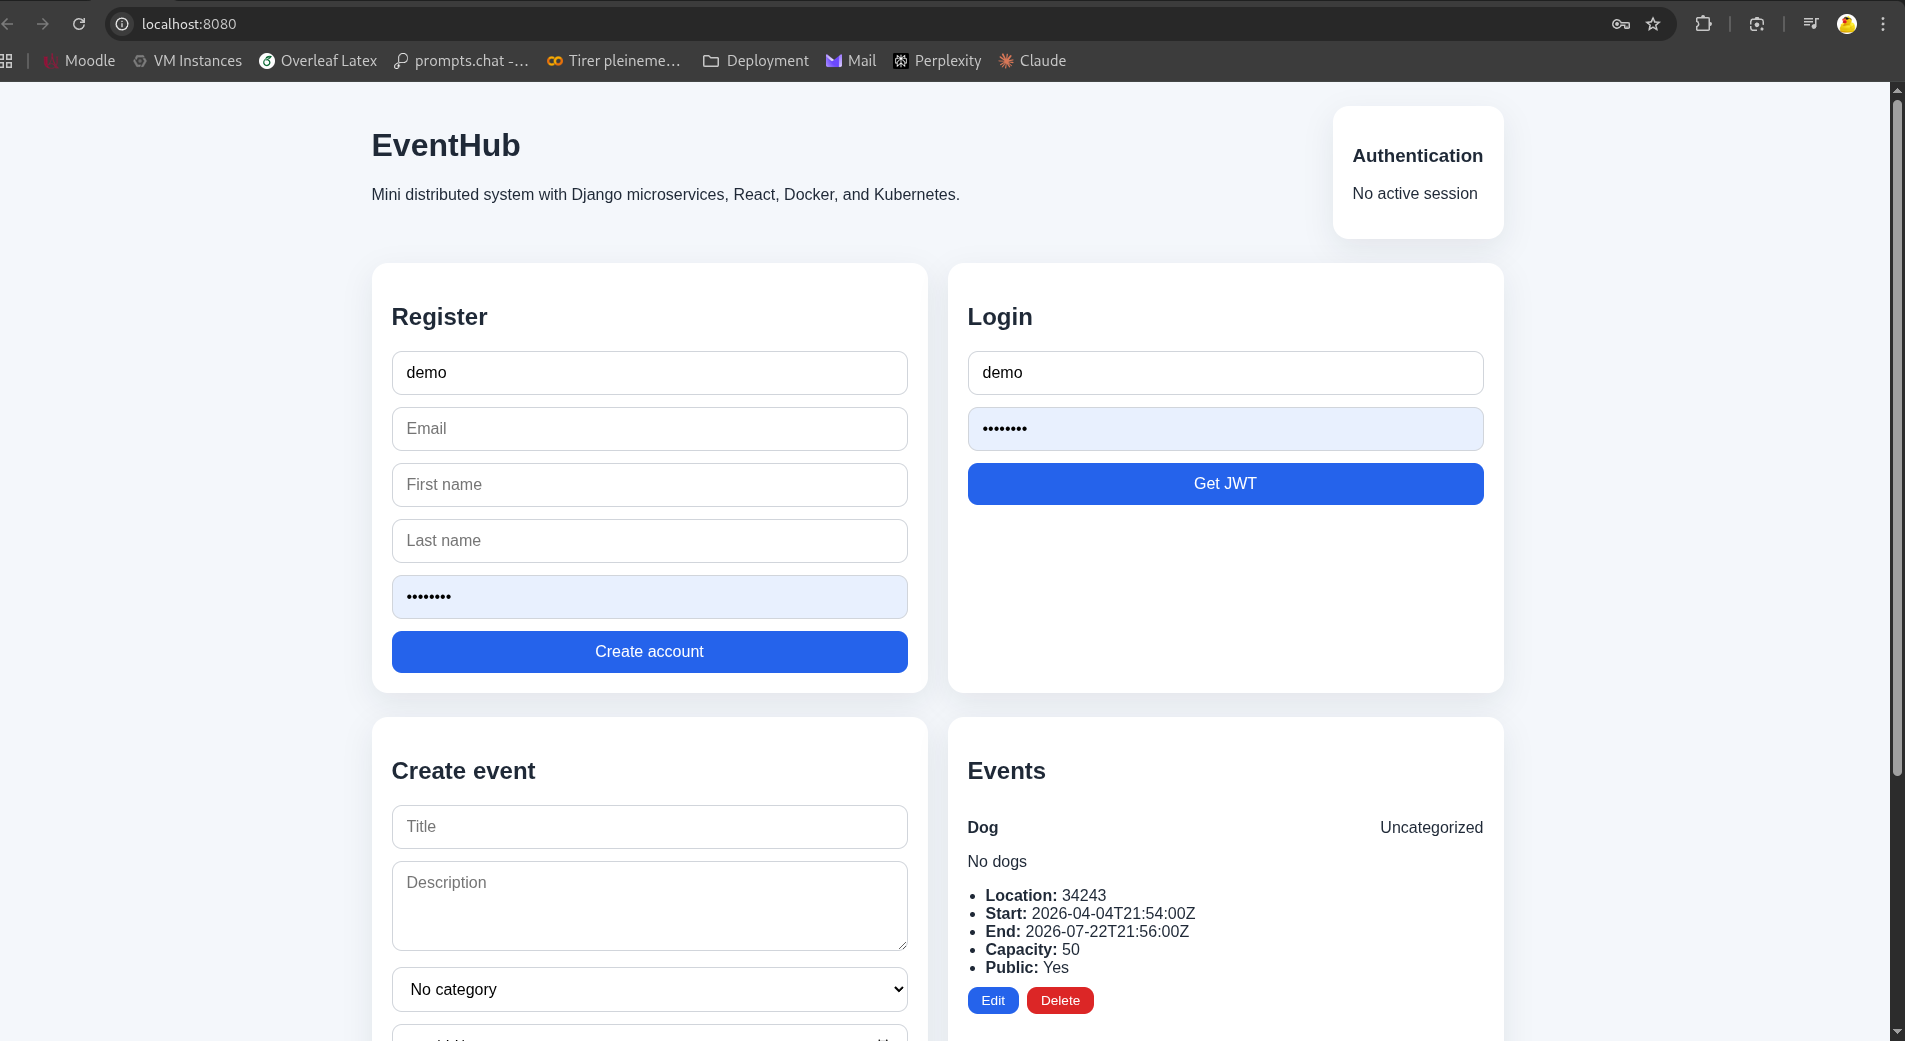
\includegraphics[width=\linewidth]{assets/screen-04-browser-frontend.png}
  \caption{Frontend EventHub accessible via la gateway sur \code{http://localhost:8080} (Docker Compose).}
\end{figure}

% ====================================================
\section{Palier 14/20 : un deuxième microservice}

\subsection{Le service \code{user-service}}

Le \code{user-service} gère l'authentification et les comptes utilisateurs. Il utilise le modèle \code{User} standard de Django et expose des endpoints JWT fournis par \code{djangorestframework-simplejwt} :

\begin{itemize}
    \item \code{POST /users/auth/register/} -- création de compte
    \item \code{POST /users/auth/login/} -- émission d'un couple access/refresh
    \item \code{POST /users/auth/refresh/} -- rafraichissement du access token
    \item \code{GET  /users/profile/} -- profil de l'utilisateur courant (token requis)
\end{itemize}

Le service est packagé avec le même pattern que \code{event-service} : \code{Dockerfile} identique, \code{ConfigMap} dédié, \code{Secret} partagé (ils se connectent tous deux à la même instance PostgreSQL, mais sur des bases logiques différentes).

\subsection{Communication inter-services à travers la gateway}

La mise en relation des deux services se fait \textbf{via la passerelle} et non par appel backend-à-backend : le frontend, après connexion sur \code{/users/auth/login/}, stocke le JWT dans \code{localStorage} et l'attache en en-tête \code{Authorization: Bearer <token>} sur les requêtes suivantes vers \code{/events/}. Ce découplage donne deux propriétés intéressantes :

\begin{enumerate}
    \item les services n'ont aucune dépendance de compile-time l'un envers l'autre ;
    \item un changement d'adresse ou de déploiement d'un service est transparent pour l'autre, la gateway servant de couche d'indirection.
\end{enumerate}

\begin{figure}[H]
  \centering
  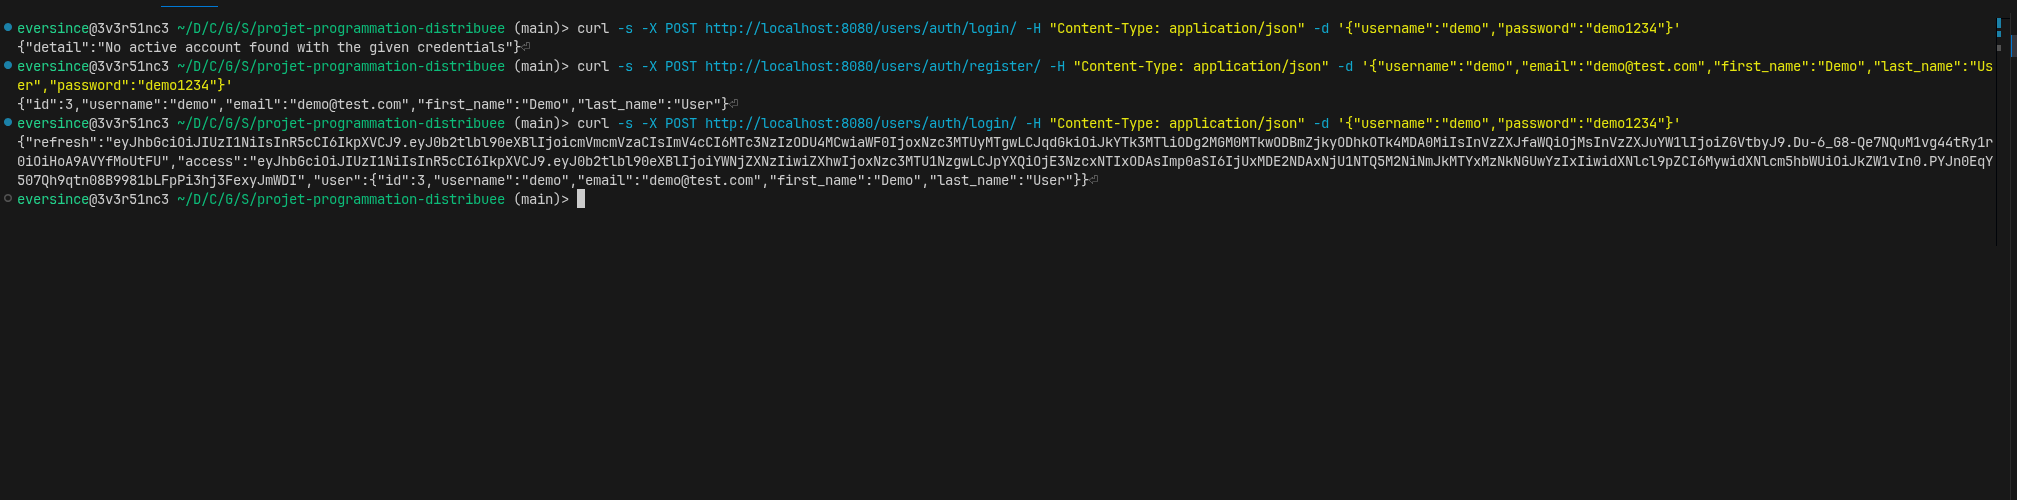
\includegraphics[width=\linewidth]{assets/screen-05-curl-jwt.png}
  \caption{Appel \code{curl} au login (obtention du JWT) puis requête authentifiée sur \code{/events/}.}
\end{figure}

% ====================================================
\section{Palier 16/20 : base de données}

\subsection{PostgreSQL comme service d'état}

La persistance est assurée par une instance PostgreSQL 16 en Alpine, déployée en Kubernetes sous forme de \code{StatefulSet} mono-réplica. L'état est conservé dans un \code{PersistentVolume} de type \code{hostPath} (adapté à Minikube) relié au pod via un \code{PersistentVolumeClaim} :

\begin{lstlisting}[caption={Extrait de \code{k8s/postgres-statefulset.yaml}}]
spec:
  containers:
    - name: postgres
      image: postgres:16-alpine
      env:
        - name: POSTGRES_USER
          valueFrom:
            secretKeyRef: { name: postgres-secret, key: POSTGRES_USER }
        - name: POSTGRES_PASSWORD
          valueFrom:
            secretKeyRef: { name: postgres-secret, key: POSTGRES_PASSWORD }
      volumeMounts:
        - name: postgres-storage
          mountPath: /var/lib/postgresql/data
        - name: postgres-init
          mountPath: /docker-entrypoint-initdb.d
  volumes:
    - name: postgres-storage
      persistentVolumeClaim: { claimName: postgres-pvc }
    - name: postgres-init
      configMap: { name: postgres-init-config }
\end{lstlisting}

\subsection{Cloisonnement logique par base}

Plutôt que de déployer deux instances PostgreSQL -- ce qui complexifierait l'infrastructure sans gain pédagogique -- nous avons fait le choix d'\emph{une} instance avec \emph{deux bases logiques} :

\begin{itemize}
    \item \code{eventhub\_events} (utilisée par \code{event-service})
    \item \code{eventhub\_users} (utilisée par \code{user-service})
\end{itemize}

Ces deux bases, ainsi que leurs utilisateurs applicatifs respectifs avec des mots de passe distincts, sont créées automatiquement au premier démarrage via un script \code{init.sql} monté dans \code{/docker-entrypoint-initdb.d} par un \code{ConfigMap}. Chaque service ne dispose que des identifiants de sa propre base, ce qui limite le rayon d'impact d'un éventuel compromis.

\begin{figure}[H]
  \centering
  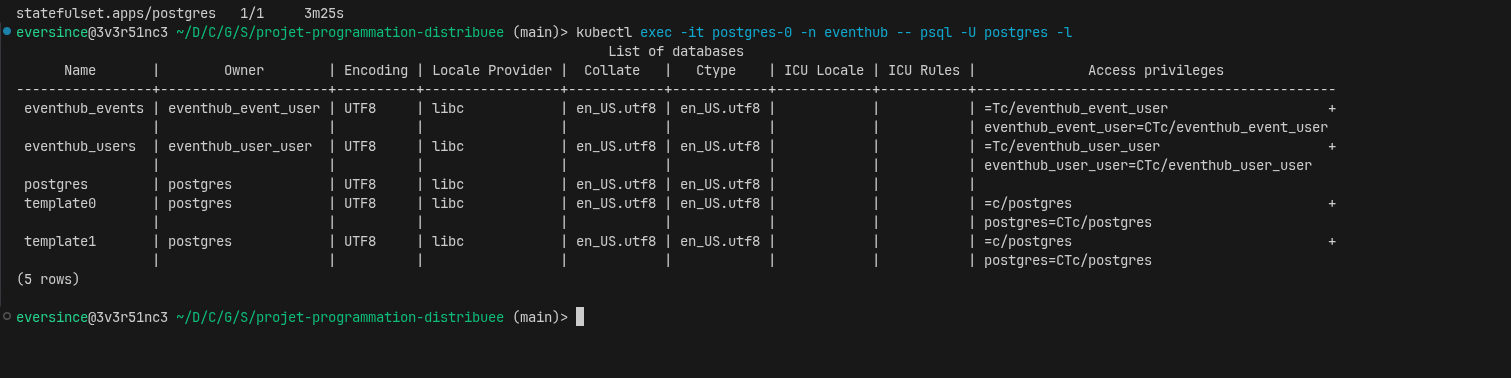
\includegraphics[width=\linewidth]{assets/screen-06-psql-databases.png}
  \caption{\code{kubectl exec postgres-0 -n eventhub -- psql -U postgres -l} -- les deux bases logiques \code{eventhub\_events} et \code{eventhub\_users}.}
\end{figure}

% ====================================================
\section{Palier 18/20 : éléments de sécurité du cluster}

Le palier 18/20 vise la sécurisation du cluster Kubernetes. Les éléments intégrés dans EventHub sont les suivants :

\subsection{Secrets Kubernetes}

Aucun mot de passe n'est stocké en clair dans les manifestes de déploiement. Les identifiants de la base de données sont centralisés dans un objet \code{Secret} (\code{k8s/postgres-secret.yaml}) et référencés par \code{secretKeyRef}. Le dépôt Git ne contient que des valeurs d'exemple ; la version réelle est générée à partir d'un \code{.env} non versionné.

\subsection{Exposition restreinte des services}

Seul l'Ingress est public. Les trois \code{Service} backend (\code{event-service}, \code{user-service}, \code{frontend-service}) sont définis en \code{ClusterIP} et n'ont pas d'IP externe. De même, \code{postgres} est en \code{ClusterIP} dans un \code{StatefulSet} \emph{headless}, accessible uniquement depuis les pods applicatifs du namespace \code{eventhub}.

\subsection{RBAC}

Un premier niveau de RBAC est fourni par \code{k8s/rbac-viewer.yaml} :

\begin{lstlisting}[caption={Rôle lecture seule sur le namespace}]
kind: Role
metadata: { name: eventhub-read-role, namespace: eventhub }
rules:
  - apiGroups: [""]
    resources: ["pods", "services", "configmaps", "secrets"]
    verbs: ["get", "list", "watch"]
  - apiGroups: ["apps"]
    resources: ["deployments", "statefulsets", "replicasets"]
    verbs: ["get", "list", "watch"]
\end{lstlisting}

Ce \code{Role} est lié via un \code{RoleBinding} à un \code{ServiceAccount} \code{eventhub-viewer} qui peut ainsi inspecter le namespace sans possibilité de modification. C'est le schéma minimal attendu par la consigne \emph{« ajouter des RBAC Kubernetes »} du sujet.

\subsection{Namespace dédié}

L'ensemble des objets est isolé dans le namespace \code{eventhub}. Cela facilite l'application de politiques transverses (RBAC, quotas, NetworkPolicies) et évite toute interférence avec les namespaces système.

\begin{figure}[H]
  \centering
  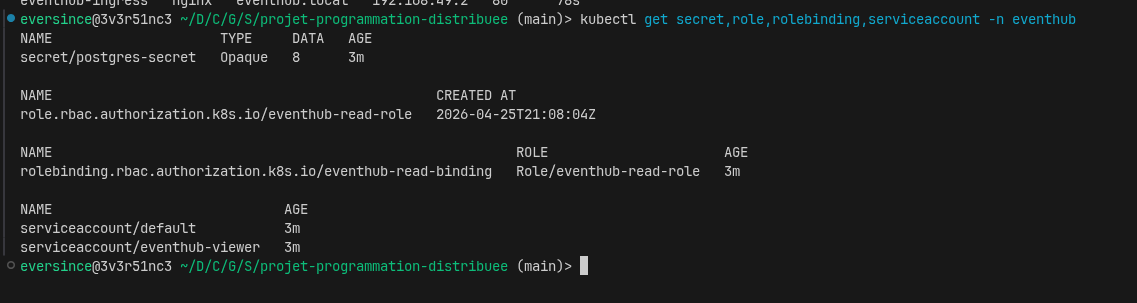
\includegraphics[width=\linewidth]{assets/screen-07-kubectl-rbac.png}
  \caption{\code{kubectl get secret,role,rolebinding,sa -n eventhub} -- objets RBAC appliqués.}
\end{figure}

% ====================================================
\section{Palier 20/20 : déploiement cloud (bonus)}

Le dernier palier du sujet récompense un déploiement dans une infrastructure cloud. L'ensemble des manifestes Kubernetes du projet est écrit de manière compatible avec une cible managée (GKE, AKS, EKS) : aucun objet ne dépend de Minikube au-delà du \code{PersistentVolume} de type \code{hostPath}, qu'il suffit de remplacer par un \code{StorageClass} dynamique (par exemple \code{standard-rwo} sur GKE).

La procédure de bascule GKE, validée par nos labs Google Cloud (voir captures individuelles en annexe du courriel de rendu), est la suivante :

\begin{enumerate}
    \item création d'un cluster Autopilot : \\
          \code{gcloud container clusters create-auto eventhub --region=europe-west1}
    \item pousser les images dans Artifact Registry et adapter le champ \code{image:} des \code{Deployment} ;
    \item remplacer le \code{PersistentVolume} \code{hostPath} par une déclaration \code{storageClassName: standard-rwo} ;
    \item appliquer les manifestes tels quels : \code{kubectl apply -f k8s/} ;
    \item récupérer l'IP publique de l'Ingress et pointer l'hôte \code{eventhub.local}.
\end{enumerate}

Les captures d'écran individuelles des profils Google Cloud Skills Boost (une par membre du trinôme) sont jointes au courriel de rendu, conformément à la consigne du sujet.

% ====================================================
\section{Mise en œuvre et démonstration}

\subsection{Lancement local par Docker Compose}

Pour la démonstration la plus rapide, le projet tourne en local avec :

\begin{lstlisting}[language=bash]
cp .env.example .env
docker compose up --build
# puis :
#   http://localhost:8080/          (frontend via gateway)
#   http://localhost:8080/events/
#   http://localhost:8080/users/auth/login/
\end{lstlisting}

Le fichier \code{docker-compose.yml} orchestre les cinq conteneurs (\code{postgres}, \code{event-service}, \code{user-service}, \code{frontend-service}, \code{gateway}) sur un réseau bridge isolé \code{eventhub-net}, avec volume nommé \code{postgres\_data} pour la persistance.

\subsection{Déploiement Kubernetes (Minikube)}

\begin{lstlisting}[language=bash]
minikube start
minikube addons enable ingress

eval $(minikube docker-env)
docker build -t eventhub-event-service:latest    ./services/event-service
docker build -t eventhub-user-service:latest     ./services/user-service
docker build -t eventhub-frontend-service:latest ./services/frontend-service

kubectl apply -f k8s/namespace.yaml
kubectl apply -f k8s/postgres-secret.yaml   -f k8s/postgres-configmap.yaml
kubectl apply -f k8s/postgres-pv.yaml       -f k8s/postgres-pvc.yaml
kubectl apply -f k8s/postgres-service.yaml  -f k8s/postgres-statefulset.yaml
kubectl apply -f k8s/event-configmap.yaml   -f k8s/user-configmap.yaml
kubectl apply -f k8s/frontend-configmap.yaml
kubectl apply -f k8s/event-deployment.yaml  -f k8s/event-service.yaml
kubectl apply -f k8s/user-deployment.yaml   -f k8s/user-service.yaml
kubectl apply -f k8s/frontend-deployment.yaml -f k8s/frontend-service.yaml
kubectl apply -f k8s/rbac-viewer.yaml       -f k8s/ingress.yaml

echo "$(minikube ip) eventhub.local" | sudo tee -a /etc/hosts
\end{lstlisting}

\begin{figure}[H]
  \centering
  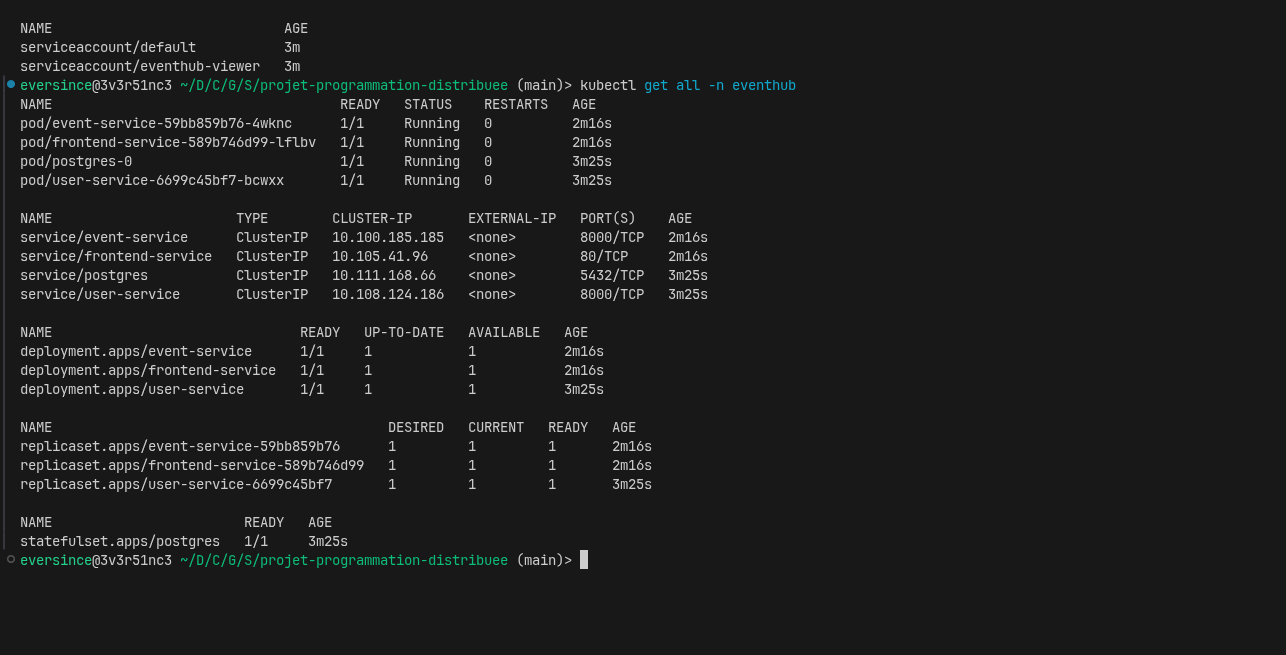
\includegraphics[width=\linewidth]{assets/screen-08-kubectl-all.png}
  \caption{\code{kubectl get all -n eventhub} -- tous les objets en état \code{Running} / \code{Ready}.}
\end{figure}

\begin{figure}[H]
  \centering
  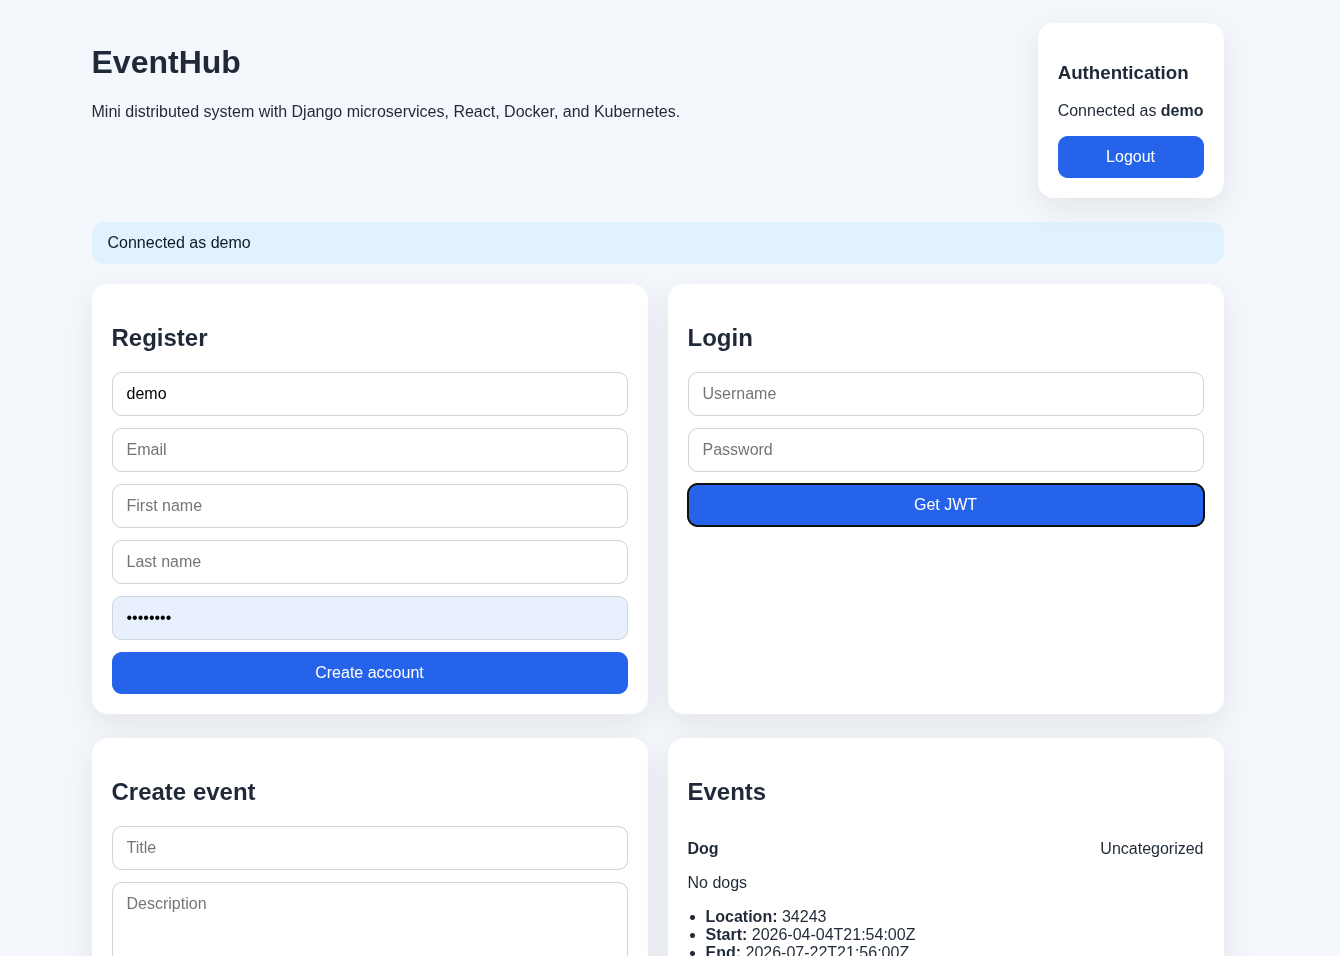
\includegraphics[width=\linewidth]{assets/screen-09-frontend-events.png}
  \caption{Interface EventHub après connexion JWT -- liste des évènements chargée depuis l'API.}
\end{figure}

% ====================================================
\section{Évaluation selon les critères du sujet}

Le sujet liste quatre critères d'évaluation par ordre décroissant d'importance. Nous reprenons chacun d'entre eux.

\subsection{Intégration d'un maximum de technologies}

Technologies imposées effectivement intégrées : \emph{Web Services REST} (Django REST Framework côté backend, \code{fetch} côté frontend), \emph{Docker} (trois \code{Dockerfile}, image PostgreSQL officielle, \code{docker-compose.yml} complet), \emph{Kubernetes} (19 manifestes YAML : namespace, deployments, services, statefulset, PV/PVC, configmaps, secret, ingress, RBAC). Technologies optionnelles : \emph{frontend moderne} (React + Vite), \emph{ingress} (NGINX), \emph{gateway locale} (Nginx reverse proxy), \emph{RBAC}.

Technologies non intégrées, à discuter honnêtement : pas de gRPC (tous les échanges sont REST), pas de \emph{service mesh} type Istio (les mTLS ne sont donc pas activés), pas de déploiement cloud effectif à la date de rédaction (les manifestes sont prêts mais le cluster GKE n'est pas permanent). Ces trois points constituent le pas supplémentaire vers 20/20.

\subsection{Codage}

Le code applicatif est organisé en trois services Python/React structurés en packages Django standards (\code{events}, \code{accounts}) et en composants React (\code{App.jsx}, \code{api.js}). Les modèles, sérialiseurs et vues sont séparés, la logique JWT est isolée dans un sérialiseur dédié \code{CustomTokenObtainPairSerializer}, et les migrations Django sont générées et versionnées.

\subsection{Fonctionnalités}

Les fonctionnalités listées au paragraphe \emph{Contexte fonctionnel} sont toutes livrées et testables bout-en-bout depuis le frontend. Un utilisateur peut s'inscrire, se connecter, créer une catégorie, créer un évènement rattaché à cette catégorie, et voir ses évènements listés sur la page d'accueil.

\subsection{Présentation (front office / CSS)}

Le frontend utilise une feuille de style \code{styles.css} maison (sans framework UI lourd) qui assure une lisibilité correcte des formulaires et de la liste d'évènements. Nous reconnaissons que ce point est le moins ambitieux du projet -- l'effort a été concentré sur l'infrastructure, qui est le premier critère d'évaluation du sujet.

% ====================================================
\section{Limites et perspectives}

Nous listons ici ce qui n'a volontairement pas été fait, avec les raisons :

\begin{itemize}
    \item \textbf{Pas de gRPC}. Les deux backends sont en Python/Django ; basculer une partie du trafic en gRPC aurait ajouté une complexité (génération de stubs, gestion de deux couches de transport) peu justifiée tant qu'un seul canal REST suffit. C'est le candidat naturel pour un prolongement.
    \item \textbf{Pas de service mesh (Istio, Linkerd)}. Le sujet mentionne explicitement mTLS et service mesh dans le palier 18/20 ; nous avons couvert RBAC et \code{Secret} mais pas mTLS. L'intégration d'Istio demande une configuration non triviale du contrôle-plane et aurait pu nuire à la stabilité de la démo.
    \item \textbf{Pas de \code{NetworkPolicy}}. La segmentation réseau pourrait être renforcée (par exemple interdire aux pods frontend de parler directement à PostgreSQL, ce qu'ils ne font déjà pas par construction).
    \item \textbf{Pas de CI/CD}. Le build et la publication des images sont manuels. Un pipeline GitHub Actions serait un ajout naturel.
    \item \textbf{Couverture de tests limitée}. Les vues REST sont testables via \code{pytest-django} mais la couverture automatisée n'a pas été industrialisée.
\end{itemize}

% ====================================================
\section{Utilisation d'outils d'IA}

Nous avons utilisé l'assistant Claude (Anthropic) pour accélérer certaines tâches à fort coût d'ingénierie et faible valeur pédagogique : génération du squelette de manifestes Kubernetes à partir du schéma d'architecture, revue de la configuration Nginx de la gateway, mise en forme de ce rapport. Le travail personnel du trinôme a porté sur la conception fonctionnelle et architecturale, l'écriture et l'adaptation du code applicatif (modèles Django, vues REST, interactions JWT, composants React), l'intégration des services, la validation bout-en-bout et la rédaction du contenu analytique et argumentaire du présent document.

% ====================================================
\section{Conclusion}

EventHub couvre l'ensemble de la chaîne demandée par le sujet de Programmation distribuée : deux microservices métier indépendants, un frontend qui les consomme à travers une gateway unique, une persistance PostgreSQL déployée en \code{StatefulSet} avec \code{PersistentVolume}, des secrets Kubernetes proprement gérés, et un premier niveau de RBAC. L'architecture retenue est volontairement symétrique entre Docker Compose (pour le développement local) et Kubernetes (pour la cible cluster), ce qui réduit le coût cognitif du va-et-vient entre les deux environnements et rend la démo reproductible.

Sur la grille d'évaluation du sujet, nous positionnons le livrable autour de \textbf{16--18/20} : les paliers 10, 12, 14 et 16 sont pleinement atteints et documentés (services, gateway, persistance), le palier 18 est couvert sur ses éléments principaux (Secrets, RBAC, isolation par namespace, exposition restreinte) et partiellement sur les éléments mesh / mTLS. Le palier 20, conditionné au déploiement cloud effectif et/ou au durcissement complet, est à portée moyennant la bascule GKE décrite au paragraphe dédié et détaillée dans les captures Google labs jointes au courriel de rendu.

% ====================================================
\renewcommand{\refname}{Références}
\begin{thebibliography}{9}
\addcontentsline{toc}{section}{Références}

\bibitem{k8sdoc}
The Kubernetes Authors. \emph{Kubernetes Documentation -- Concepts}. \url{https://kubernetes.io/docs/concepts/}

\bibitem{k8srbac}
The Kubernetes Authors. \emph{Using RBAC Authorization}. \url{https://kubernetes.io/fr/docs/reference/access-authn-authz/rbac/}

\bibitem{charroux-k8s}
Charroux, B. \emph{kubernetes-minikube}. \url{https://github.com/charroux/kubernetes-minikube}

\bibitem{charroux-cwk}
Charroux, B. \emph{CodingWithKubernetes}. \url{https://github.com/charroux/CodingWithKubernetes}

\bibitem{charroux-mesh}
Charroux, B. \emph{servicemesh-kubernetes}. \url{https://github.com/charroux/servicemesh-kubernetes}

\bibitem{charroux-rental}
Charroux, B. \emph{rentalservice -- istio-internal-gateway}. \url{https://github.com/charroux/rentalservice/blob/main/k8s/base/istio-internal-gateway.yaml}

\bibitem{djangorest}
Django Software Foundation. \emph{Django REST Framework}. \url{https://www.django-rest-framework.org/}

\bibitem{simplejwt}
\emph{Simple JWT -- A JSON Web Token authentication plugin for DRF}. \url{https://django-rest-framework-simplejwt.readthedocs.io/}

\bibitem{postgresdocker}
PostgreSQL Global Development Group. \emph{Official PostgreSQL Docker image}. \url{https://hub.docker.com/_/postgres}

\bibitem{nginx}
NGINX Inc. \emph{NGINX reverse proxy documentation}. \url{https://nginx.org/en/docs/http/ngx_http_proxy_module.html}

\bibitem{istio-mtls}
Istio Authors. \emph{Mutual TLS Migration}. \url{https://istio.io/latest/docs/tasks/security/authentication/mtls-migration/}

\end{thebibliography}

\end{document}
